\documentclass{CUCProposal}

% 使用该宏包可以为参考文献、图表、公式添加超链接。但是可能会影响观感,可根据需要自行选择是否使用。
% 默认样式:使用方框标识超链接,很多期刊论文中有用
\usepackage[]{hyperref}
% 简化样式:不用方框,看起来会简洁一点,有各种颜色标识不同的类别
% \usepackage[colorlinks,linkcolor=red,anchorcolor=blue,citecolor=green]{hyperref}
% 保险样式:都是黑色的超链接,可以点击
% \usepackage[colorlinks,linkcolor=black,anchorcolor=black,citecolor=black,urlcolor=black]{hyperref}

% 中文占位符,可删除
\usepackage{zhlipsum}

% 参考文献文件位置
\addbibresource{ref.bib}

% 个人信息设置
\setup{
  % 姓名
  Name = 王小帅,
  % 学号
  StudentID = 201111111111111,
  % 责任导师
  Advisor = 王大帅,
  % 培养单位
  Department = 信息与通信工程学院,
  % 领域及代码
  Subject = 信息与通信工程0810,
  % 研究方向
  SubSubject = 智能媒体大数据,
  % 论文标题
  Title = 基于BSC模板的表格类文件 \LaTeX 实现方法研究,
  % 导师pdf电子签名
  AdvisorSign = {
\includegraphics[width=3cm]{Albus}},
  % 申请日期
  Date = 2022年12月25日
}

% 正文
\begin{document}

% 需要填写的三个部分分别为:文献综述、选题报告、导师意见,文献综述和选题报告都可以正常使用\section等命令分点论述,并且两部分的的标题独立编号。
% 由于文档不会特别长,文中的图表公式只用了 图 1 表 1 的表示
\makeKTtable{
% =====================文献综述=====================
  \section{某一个方面}
  \zhlipsum[1]
  一些文字\cite{xiangtuzhongguo}
  \subsection{其中一个点}
  \zhlipsum[2]
  一些文字\cite{rengongzhinengtongxinlilunyufangfa}
  \subsection{另一个点}
  \zhlipsum[3]
  \section{另一个方面}
  \zhlipsum[4]
  \zhlipsum[5]
% =====================文献综述=====================
}
{
% =====================选题报告=====================
  选题报告至少应包括以下方面:
  \begin{enumerate}
    \item 选题依据
    \item 创新性
    \item 选题难度和可行性
    \item 研究工作方案
    \item 科研工作时间安排
  \end{enumerate}

  \section{选题依据}

  适当引用文献\cite{rengongzhinengjianshi},适当引用文献\cite{zhongguozhexueshi},,适当引用文献\cite{jiqixuexi},适当引用文献\cite{vaswani_attention_2017},序号与本报告最后的参考文献一致。

  \section{研究工作方案}

  \subsection{研究技术路线}

  \noindent
  \begin{center}
    \begin{minipage}{0.8\linewidth}
    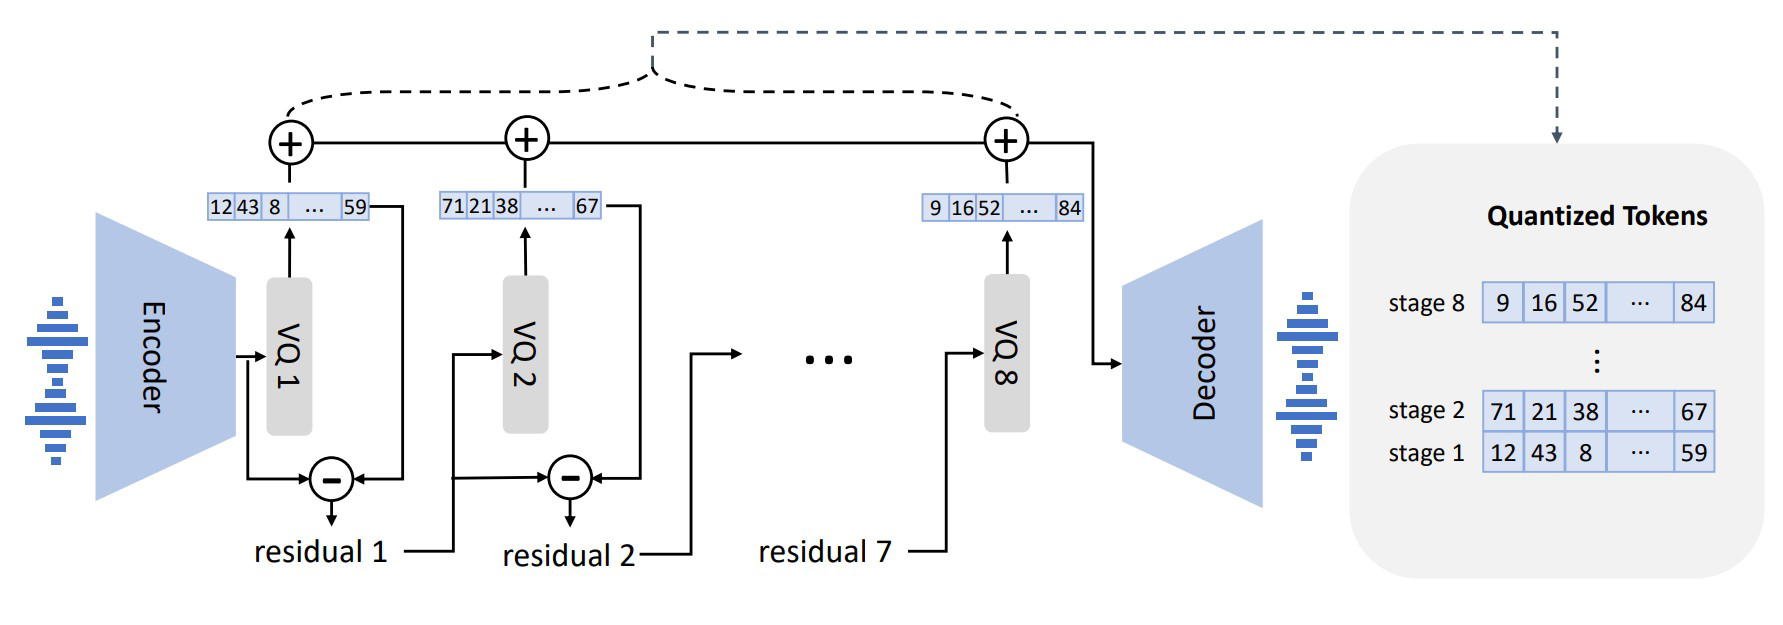
\includegraphics[width=\textwidth]{pic/VALL-E编码模型}
    \captionof{figure}{VALL-E编码模型\label{fig:examplefig}}
    \end{minipage}
  \end{center}

  \begin{center}
    \singlespacing
    \begin{minipage}{.5\linewidth}
      \begin{center}
        \captionof{table}{An example table\label{tab:exampletable}}
        \begin{tblr}{colspec={ll},hline{1,2,Z}}
          Name&Schoolo\\
          Harry Potter&Gryffindor\\
          Draco Malfoy&Slytherin\\
        \end{tblr}
      \end{center}
    \end{minipage}      
  \end{center}

  注意!文中出现的图片、表格、公式等,都需要在文中进行引用!如图\ref{fig:examplefig}、表\ref{tab:exampletable}、公式\ref{eq:exampleeq}等。

  \begin{equation}
    E = mc^2 
    \label{eq:exampleeq}
  \end{equation}

  \section{参考文献}
  \printbibliography[heading=none]
  % =====================选题报告=====================
}
{
  % =====================导师意见=====================
  \zhlipsum[5]
  % =====================导师意见=====================
}
\end{document}